\textbf{Allgemeine   Anmerkung}: Nicht   alle  benutzten   Verfahren   liefern
Resultate mit  Unsicherheiten. In den  graphischen Vergleichen  der Ergebnisse
(siehe Abbildungen
\ref{fig:schallgeschwindigkeit:results},
\ref{fig:eisengehalt:results},
\ref{fig:federkonstante:federkonstante:results},
\ref{fig:federkonstante:vorspannung:results},
\ref{fig:pendel:results} und
\ref{fig:rcglied:results})
haben   diese   Resultate   sowie  allf\"allige   Startwerte   deshalb   keine
Unsicherheiten  eingetragen. Dies  bedeutet   nat\"urlich  nicht,  dass  diese
Resultate  genauer  oder  verl\"asslicher  sind (im  Gegenteil: Da  man  keine
Angaben  \"uber  die  Unsicherheiten  hat,   sind  diese  Resultate  eher  mit
gr\"osserer Vorsicht zu geniessen).


%-------------------------------------------------------------------------------
\subsection{Schallgeschwindigkeit}
%-------------------------------------------------------------------------------

Die Diskussion wird sich hier v.a. um zwei Aspekte drehen:

\begin{itemize}
    \item
        Den  Vergleich zwischen  Literaturwerten und  den Ergebnissen  aus den
        Messdaten,
    \item
        sowie     den    Vergleich     der    Ergebnisse     der    ``vollen''
        Fehlerfortpflanzungsrechnung und der vereinfachten Variante.
\end{itemize}

Zur Rekapitulation nochmals die Ergebnisse zusammengefasst:

\begin{itemize}
    \item
        Literaturwert, Tabelle: $\SI{344}{\meter\per\second}$
    \item
        Formel:
        \begin{equation}
            \label{eq:schallgeschwTemperatur2}
            c_{luft} = (331.3 + 0.606 \cdot \vartheta) \si{\meter\per\second}  = \SI{345.24}{\meter\per\second} \approx \SI{345}{\meter\per\second}
        \end{equation}
    \item
        Mittlere Geschwindigkeit aus Messresultaten:
        \begin{gather*}
            \overline{c} = \SI{347.73}{\meter\per\second} \\
        \end{gather*}
    \item
        Unsicherheit, volles Gauss'sches Fehlerfortpflanzungsgesetz:
        \begin{equation*}
            s_{\overline{c(s,t)}} = \SI{2.93}{\meter\per\second}
        \end{equation*}
    \item
        Unsicherheit, Kurzformel f\"ur Fehlerfortpflanzung in Multiplikation/Division:
        \begin{equation*}
            s_{\overline{c(s,t)}} = \SI{2.93}{\meter\per\second}
        \end{equation*}
\end{itemize}

Sinnvoll gerundet erhalten wir aus den Messergebnissen also:
\begin{equation}
    \underline{\underline{c_{luft} = \overline{c_{luft}} \pm s_{\overline{c_{luft}}} = \SI[separate-uncertainty = true]{348 \pm 3}{\meter\per\second}}}
\end{equation}

Diese  Ergebnisse  sind in  Abbildung  \ref{fig:schallgeschwindigkeit:results}
graphisch dargestellt.

\begin{figure}[ht!]
\centering
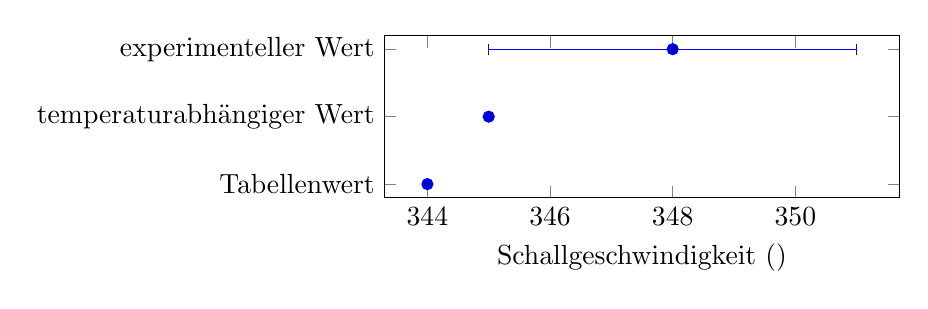
\begin{tikzpicture}
    \begin{axis}[
        width=.67\textwidth,
        height=.3\textwidth,
        %title = {Schallgeschwindigkeit, Vergleich Literaturwerte mit Experiment},
        xlabel = {Schallgeschwindigkeit ($\si{\meter\per\second}$)},
        symbolic y coords = {Tabellenwert,temperaturabh\"angiger Wert,experimenteller Wert},
    ]
    \addplot+[
        only marks,error bars/.cd,
        x dir=both,x explicit,
        error bar style={line width=0.5pt},
        ]
    coordinates {
        (344,Tabellenwert)
        (345,temperaturabh\"angiger Wert)
        (348,experimenteller Wert) +- (3,0)
    };
    \end{axis}
\end{tikzpicture}
\caption{graphische Darstellung der Ergebnisse zum Versuch \emph{Schallgeschwindigkeit}}
\label{fig:schallgeschwindigkeit:results}
\end{figure}

Es stechen dabei folgende Punkte heraus:
\begin{itemize}
    \item
        Der   Tabellenwert   stimmt  relativ   genau   mit   dem  aus   Formel
        \ref{eq:schallgeschwTemperatur2} errechneten  Wert \"uberein. Da beide
        Verfahren  aus der  Fachliteratur stammen,  ist dies  meines Erachtens
        auch zu erwarten.
    \item
        Berechnet man  die Unsicherheit der Schallgeschwindigkeit  mittels der
        Faustformel  $s_{\overline{c(s,t)}}  = \sqrt{  \left(  \frac{s_{s}}{s}
        \right)^2   +  \left(   \frac{s_{t}}{\overline{c}}  \right)^2}   \cdot
        \overline{c(s,t)}$,   ist   die   Differenz   zum   mit   dem   vollen
        Gauss'schen  Fehlerfortpflanzungsgesetz  ermittelten Werte  in  diesem
        Falle  bedeutungslos (siehe  auch Anhang~\ref{appendix:aufgabe1}). Die
        Faustformel ist also hier hinreichend genau.
        Da  die   Faustformel  im   Allgemeinen  bei   simplen  physikalischen
        Zusammenh\"angen akzeptable  Ergebnisse liefert,  ist dies  auch nicht
        weiter erstaunlich  ($c =  \frac{s}{t}$ geh\"ort sicherlich  zu dieser
        Kategorie von Gesetzm\"assigkeiten).
    \item
        Wie bereits erw\"ahnt und in Abbildung \ref{fig:schallgeschwindigkeit}
        auf Seite  \pageref{fig:schallgeschwindigkeit} ersichtlich,  liegen 13
        der  20  Messpunkte  innerhalb  des  Intervals  Mittelwert  $\pm$  die
        Standardabweichung. Dies  entspricht   einem  Anteil  von   65\%,  was
        ziemlich nahe beim theoretischen Wert  von 68\% liegt. W\"urde man die
        Anzahl (korrekt  durchgef\"uhrter) Messungen erh\"ohen,  w\"urden sich
        diese beiden Werte weiter ann\"ahern.
    \item
        Bezieht   man   die   Unsicherheit    der   aus   den   Messresultaten
        bestimmten   Schallgeschwindigkeit    mit   ein,   ist    die   untere
        Grenze  des   experimentellen  Wertes  ($\SI{345}{\meter\per\second}$)
        lediglich  $\SI{1}{\meter\per\second}$  h\"oher als  der  Tabellenwert
        von    \SI{344}{\meter\per\second},    und    der    mittels    Formel
        \ref{eq:schallgeschwTemperatur2} bestimmte Wert  liegt sogar innerhalb
        des Unsicherheitsbereichs.
        F\"ur die verbleibende Differenz vermute ich folgende Gr\"unde:
        \begin{itemize}
            \item
                Die  Werte  aus  der Fachliteratur  haben  keine  Unsicherheit
                angegeben. Es   ist   also   durchaus  m\"oglich,   dass   bei
                Ber\"ucksichtigung   dieser    Unsicherheit   die   Intervalle
                der    Literaturwerte   inklusive    Unsicherheit   mit    den
                hier   bestimmten    experimentellen   Ergebnissen   inklusive
                Unsicherheiten \"uberlappen.
            \item
                Die Anzahl Messpunkte des Tabellenwertes aus der Fachliteratur
                ist vermutlich h\"oher.
            \item
                Die Werte  aus der  Fachliteratur wurden  m\"oglicherweise mit
                teureren  (genaueren)  Messaparaten  bestimmt   als  die  hier
                vorliegenden Daten.
            \item
                Die Werte aus der  Fachliteratur wurden m\"oglicherweise unter
                besser  kontrollierten  Bedingungen   gemessen  als  die  hier
                vorliegenden Daten.
            \item
                Die Werte aus der  Fachliteratur wurden m\"oglicherweise mit
                anderen Methoden bestimmt als der hier ausgef\"uhrte Versuch.
        \end{itemize}
\end{itemize}

Alles  in allem  ist  das  Resultat aus  diesem  Versuch  meiner Ansicht  nach
ziemlich gut, die Resultate plausibel und von zufriedenstellender Qualit\"at.

%\begin{center}
%\begin{tikzpicture}
%\begin{axis}[xbar,enlargelimits=0.15]
%\addplot
%[draw=blue,pattern=horizontal lines light blue]
%coordinates
%    {(10,5) (15,10) (5,15) (24,20) (30,25)};
%
%\addplot
%[draw=black,pattern=horizontal lines dark blue]
%coordinates
%    {(3,5) (5,10) (15,15) (20,20) (35,25)};
%\end{axis}
%\end{tikzpicture}

%\begin{tikzpicture}
%\begin{axis}
%\addplot+[only marks,scatter,error bars/.cd,
%    y dir=both,y explicit,
%    x dir=both,x fixed=0.05,
%    error mark=diamond*]
%coordinates {
%    (0,0) +- (0.5,0.1)
%    (0.1,0.1) +- (0.05,0.2)
%    (0.2,0.2) +- (0,0.05)
%    (0.5,0.5) +- (0.1,0.2)
%    (1,1) +- (0.3,0.1)};
%\end{axis}
%\end{tikzpicture}


\clearpage
%-------------------------------------------------------------------------------
\subsection{Eisengehalt}
%-------------------------------------------------------------------------------

Die   erhaltenen   Werte   tabellarisch   und   graphisch   (siehe   Abbildung
\ref{fig:eisengehalt:results}) zusammengefasst:

\begin{center}
\begin{tabular}{lrrr}
    \toprule
                     & ungewichtet                   & gewichtet                     & QtiPlot, gewichtet            \\
    \midrule
    Mittelwert       & $\SI{20.44}{\percent}$        & $\SI{20.37}{\percent}$        & $\SI{20.37}{\percent}$        \\
    Unsicherheit     & $\SI{ 0.46}{\percent}$        & $\SI{ 0.36}{\percent}$        & $\SI{ 0.36}{\percent}$        \\
    \midrule
    Gerundet         & $\SI{20.4 \pm 0.5}{\percent}$ & $\SI{20.4 \pm 0.4}{\percent}$ & $\SI{20.4 \pm 0.4}{\percent}$ \\
    \bottomrule
\end{tabular}
\end{center}

\vspace*{2em}
\begin{figure}[ht!]
\centering
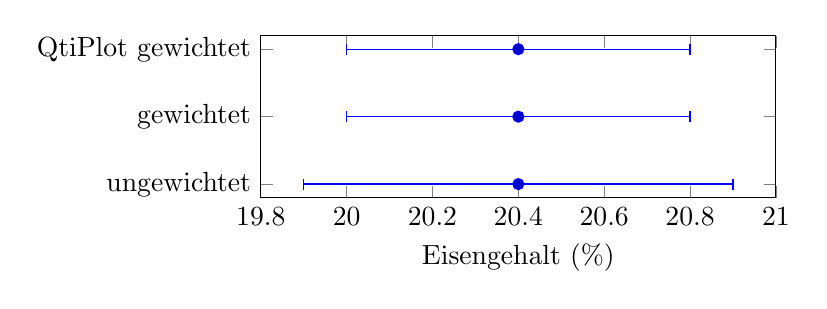
\begin{tikzpicture}
    \begin{axis}[
        width=.67\textwidth,
        height=.3\textwidth,
        %title = {Eisengehalt},
        xlabel = {Eisengehalt (\%)},
        symbolic y coords = {ungewichtet,gewichtet, QtiPlot gewichtet},
    ]
    \addplot+[
        only marks,error bars/.cd,
        x dir=both,x explicit,
        error bar style={line width=0.5pt},
        ]
    coordinates {
        (20.4,ungewichtet) +- (0.5,0)
        (20.4,gewichtet) +- (0.4,0)
        (20.4,QtiPlot gewichtet) +- (0.4,0)
    };
    \end{axis}
\end{tikzpicture}
\caption{graphische Darstellung der Ergebnisse zum Versuch \emph{Schallgeschwindigkeit}}
\label{fig:eisengehalt:results}
\end{figure}

Der   Unterschied   zwischen    gewichteten   Resultaten   und   ungewichteten
Resultaten    ist    hier    beim    Mittelwert    nicht    besonders    gross
(Abweichungen   im   Promillebereich: $1-\frac{20.37}{20.44}  \approx   0.003$
btw. $1-\frac{20.44}{20.36}  \approx -0.003$).   Die  relative Abweichung  bei
der Unsicherheit  ist hingegen  gr\"osser ($1-\frac{0.36}{0.46}  \approx 0.22$
bzw. $1-\frac{0.46}{0.36} \approx -0.28$). Jedoch ist diese Abweichung im Vergleich
zum Mittelwert immer noch nicht besonders hoch.

Ob diese  Abweichungen von Bedeutung sind, h\"angt schlussendlich nat\"urlich
davon ab, wof\"ur diese Resultate verwendet werden sollen.

Es ist  ebenfalls eine  gute \"Ubereinstimmung mit  den von  QtiPlot bestimten
Werten  festzustellen  (siehe   Abbildungen  \ref{fig:eisengehalt}  auf  Seite
\pageref{fig:eisengehalt} und \ref{fig:eisengehalt:results}).


\clearpage
%-------------------------------------------------------------------------------
\subsection{Federkonstante}
%-------------------------------------------------------------------------------

Die Resultate tabellarisch und graphisch zusammengefasst:

\begin{center}
\begin{tabular}{lrrr}
    \toprule
                                    & Handrechnung/Spreadsheet             & TI-89 & QtiPlot                                \\
    \midrule
    Federkonstante $k$              & $\SI{22.6}{\newton\per\meter}$ & $\SI{22.3}{\newton\per\meter}$ & $\SI{22.3 \pm 0.9}{\newton\per\meter}$ \\
    Vorspannung $F_0$               & $\SI{-0.7}{\newton}$           & $\SI{-0.5}{\newton}$           & $\SI{-0.5 \pm 0.5}{\newton}$           \\
    empirische Korrelation $r_{xy}$ & $0.99364$                       & $0.993638$                     & k.A.                                   \\
    Bestimmtheitsmass $R^2$         & $0.98732$                       & $0.987316$                     & $0.9873$                               \\
    \bottomrule
\end{tabular}
\end{center}

\vspace*{2em}
\begin{figure}[ht!]
\centering
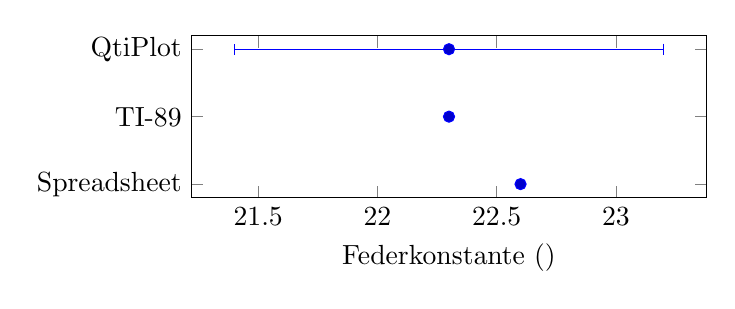
\begin{tikzpicture}
    \begin{axis}[
        width=.67\textwidth,
        height=.3\textwidth,
        %title = {Federkonstante},
        xlabel = {Federkonstante ($\si{\newton\per\meter}$)},
        symbolic y coords = {Spreadsheet,TI-89,QtiPlot},
    ]
    \addplot+[
        only marks,error bars/.cd,
        x dir=both,x explicit,
        error bar style={line width=0.5pt},
        ]
    coordinates {
        (22.6,Spreadsheet)
        (22.3,TI-89)
        (22.3,QtiPlot) +- (0.9,0)
    };
    \end{axis}
\end{tikzpicture}
\caption{
    Graphische    Darstellung     der    Federkonstante     zum    Versuch
    \emph{Federkonstante}. Auch  wenn  die  Methode  mittels  Spreadsheet  und
    TI-89   keine   Unsicherheiten   liefern,   liegen   sie   innerhalb   des
    Unsicherheitsbereiches   des  Resultats   von   QtiPlot,   was  ich   also
    zufriedenstellend beurteile.
}
\label{fig:federkonstante:federkonstante:results}
\end{figure}

\vspace*{2em}
\begin{figure}[ht!]
\centering
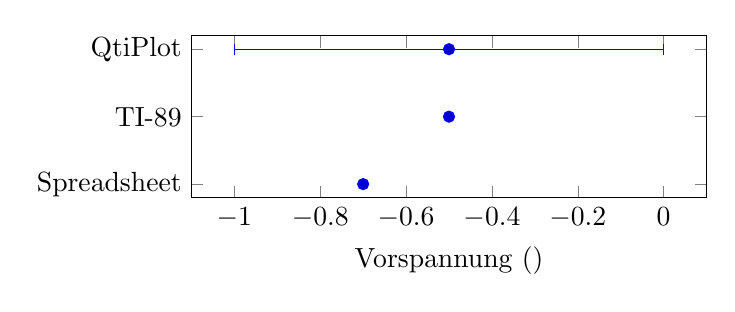
\begin{tikzpicture}
    \begin{axis}[
        width=.67\textwidth,
        height=.3\textwidth,
        %title = {Vorspannung},
        xlabel = {Vorspannung ($\si{\newton}$)},
        symbolic y coords = {Spreadsheet,TI-89,QtiPlot},
    ]
    \addplot+[
        only marks,error bars/.cd,
        x dir=both,x explicit,
        error bar style={line width=0.5pt},
        ]
    coordinates {
        (-0.7,Spreadsheet)
        (-0.5,TI-89)
        (-0.5,QtiPlot) +- (0.5,0)
    };
    \end{axis}
\end{tikzpicture}
\caption{
    Graphische      Darstellung      der     Vorspannung      zum      Versuch
    \emph{Federkonstante}. Auch  hier  liegen  die  Werte des  TI-89  und  des
    Spreadsheets  innerhalb  des   Unsicherheitsbereichts  des  Resultats  von
    QtiPlot.
}
\label{fig:federkonstante:vorspannung:results}
\end{figure}

Vergleicht  man   die  Ergebnisse   von  QtiPlot   mit  den   Ergebnissen  des
Taschenrechners, kann  man eine  sehr gute  \"Ubereinstimmung feststellen. Ich
f\"uhre  dies  darauf  zur\"uck,  dass  vermutlich  sowohl  QtiPlot  wie  auch
der  TI-89  die gleichen  Algorithmen  zur  Bestimmung der  Regressionsgeraden
verwenden. Konsequenterweise  ist es  naheliegend, dass  sie aus  den gleichen
Daten auf das gleiche Ergebnis kommen.

Ein  wesentlicher  Unterschied zwischen  QtiPlot  und  dem Taschenrechner  ist
jedoch, dass der TI-89 keine Unsicherheiten ausgibt.

Zur  Erg\"anzung und  aus  Neugier  habe ich  noch  eine  Berechnung von  Hand
bzw.  mit  Tabellenkalkulationsprogramm   durchgef\"uhrt  (siehe  auch  Anhang
\ref{appendix:aufgabe3}).

Da dieses Verfahren (zumindest soweit ich herausfinden kann) nicht der gleiche
Algorithmus  ist, wie  er  von  QtiPlot und  dem  TI-89  verwendet wird,  sind
die  damit erhaltenen  Resultate auch  nicht ganz  identisch. Sie sind  jedoch
gen\"ugend nahe, dass ich sie als plausibel beurteile und damit zufrieden bin.


%-------------------------------------------------------------------------------
\subsection{Pendel}
%-------------------------------------------------------------------------------

Zur Rekapitulation hier nochmals die Pendelgleichung mit gerundeten Parametern:
\begin{align*}
    y(t)   & = A \cdot exp(-\Gamma \cdot t) \cdot sin(2 \cdot \pi \cdot f \cdot t - \delta) + y_0 \\
           & =     \SI[separate-uncertainty = true]{1.29 \pm 0.04}{\meter}
           \cdot exp\left(\SI[separate-uncertainty = true]{-0.052 \pm 0.002}{\per\second}\right) \\
           & \cdot sin\left(2\pi \cdot \SI[separate-uncertainty = true]{0.0533 \pm 0.0003}{\hertz} \cdot t - \num[separate-uncertainty = true]{0.50 \pm 0.02}\right) \\
           & + \SI[separate-uncertainty = true]{0.041 \pm 0.007}{\meter}
\end{align*}

Die  Hauptschwierigkeit  bei  dieser  Aufgabe  liegt  darin,  gute  Startwerte
f\"ur  die nichtlineare  Regression in  QtiPlot zu  finden. Die dazu  benutzte
Verfahrensweise ist ausf\"uhrlich in Abschnitt \ref{subsec:pendel} erkl\"art.

Interessant  ist  dabei, dass  die  mit  eigentlich ziemlich  groben  Methoden
ermittelten  Startwerte  gar  nicht  so weit  von  den  anschliessend  mittels
Iteration von  QtiPlot bestimmten Werten entfernt  liegen. Eine rasche Analyse
eines Scatter-Plots mittels Augenmass und  einiger kurzer Rechnungen kann also
je  nach  Datensatz  bereits  ziemlich starke  Aussagen  \"uber  die  gesuchte
Gesetzm\"assigkeit machen.

Dies kann insbesondere bei der  Beurteilung der Plausibilit\"at der Resultate,
die von einem Computerprogramm geliefert werden, hilreich oder sogar notwendig
sein. Im vorliegenden  Falle macht mir das  Resultat einen zufriedenstellenden
Eindruck.

\begin{center}
\begin{tabular}{lrr}
    \toprule
                                & Startwert                  & Endwert \\
    \midrule
    Amplitude $A$               &  $\SI{1}{\meter}$          & $\SI{ 1.29 \pm 0.04}{\meter}$ \\
    D\"ampfung $\Gamma$         &  $\SI{0.035}{\per\second}$ & $\SI{0.052 \pm 0.002}{\per\second}$ \\
    Frequenz $f$                &  $\SI{0.05}{\hertz}$       & $\SI{ 0.0533  \pm 0.0003}{\hertz}$ \\
    Phasenverschiebung $\delta$ &  $0.31$                    & $\num{0.50  \pm 0.02}$ \\
    Anfangsauslenkung $y_0$     &  $\SI{0}{\meter}$          & $\SI{ 0.041 \pm 0.007}{\meter}$ \\
    \bottomrule
\end{tabular}
\end{center}

\begin{figure}[ht!]
\centering
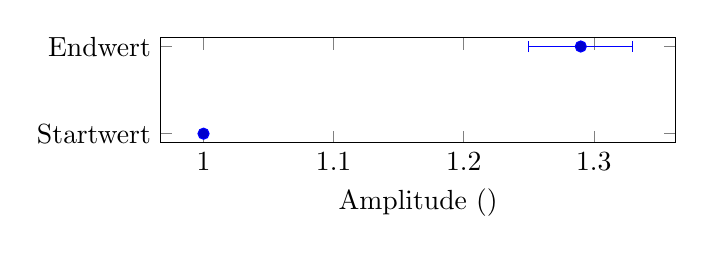
\begin{tikzpicture}
    \begin{axis}[
        try min ticks=2,
        width=.67\textwidth,
        height=.24\textwidth,
        %title = {Vergleich Startwerte und Endwerte: Amplitude},
        xlabel = {Amplitude ($\si{\meter}$)},
        symbolic y coords = {Startwert,Endwert}
    ]
    \addplot+[
        only marks,error bars/.cd,
        x dir=both,x explicit,
        error bar style={line width=0.5pt},
        ]
    coordinates {
        (1,Startwert)
        (1.29,Endwert) +- (0.04,0)
    };
    \end{axis}
\end{tikzpicture}
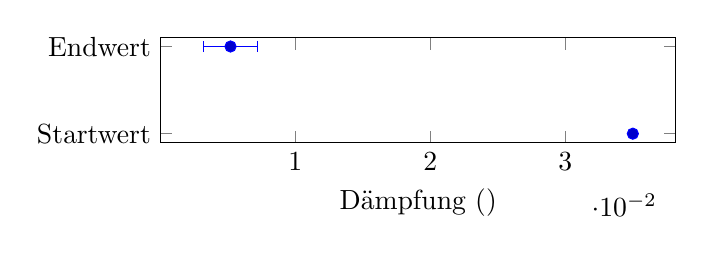
\begin{tikzpicture}
    \begin{axis}[
        try min ticks=2,
        width=.67\textwidth,
        height=.24\textwidth,
        %title = {Vergleich Startwerte und Endwerte: D\"ampfung},
        xlabel = {D\"ampfung ($\si{\per\second}$)},
        symbolic y coords = {Startwert,Endwert}
    ]
    \addplot+[
        only marks,error bars/.cd,
        x dir=both,x explicit,
        error bar style={line width=0.5pt},
        ]
    coordinates {
        (0.035,Startwert)
        (0.0052,Endwert) +- (0.002,0)
    };
    \end{axis}
\end{tikzpicture}
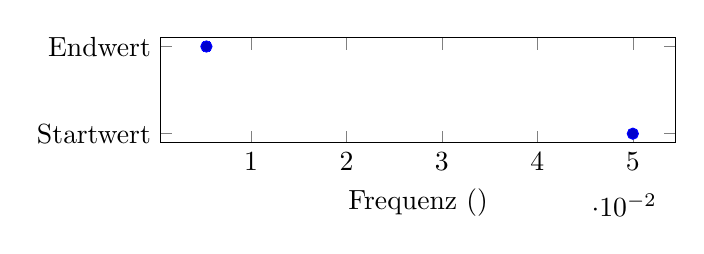
\begin{tikzpicture}
    \begin{axis}[
        try min ticks=2,
        width=.67\textwidth,
        height=.24\textwidth,
        %title = {Vergleich Startwerte und Endwerte: Frequenz},
        xlabel = {Frequenz ($\si{\hertz}$)},
        symbolic y coords = {Startwert,Endwert}
    ]
    \addplot+[
        only marks,error bars/.cd,
        x dir=both,x explicit,
        error bar style={line width=0.5pt},
        ]
    coordinates {
        (0.05,Startwert)
        (0.00533,Endwert) +- (0.0003,0)
    };
    \end{axis}
\end{tikzpicture}
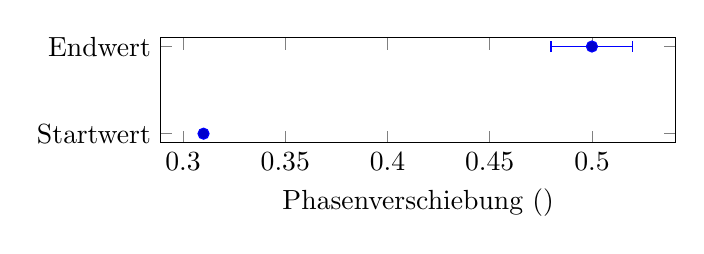
\begin{tikzpicture}
    \begin{axis}[
        try min ticks=2,
        width=.67\textwidth,
        height=.24\textwidth,
        %title = {Vergleich Startwerte und Endwerte: Phasenverschiebung},
        xlabel = {Phasenverschiebung ($\si{\radian}$)},
        symbolic y coords = {Startwert,Endwert}
    ]
    \addplot+[
        only marks,error bars/.cd,
        x dir=both,x explicit,
        error bar style={line width=0.5pt},
        ]
    coordinates {
        (0.31,Startwert)
        (0.50,Endwert) +- (0.02,0)
    };
    \end{axis}
\end{tikzpicture}
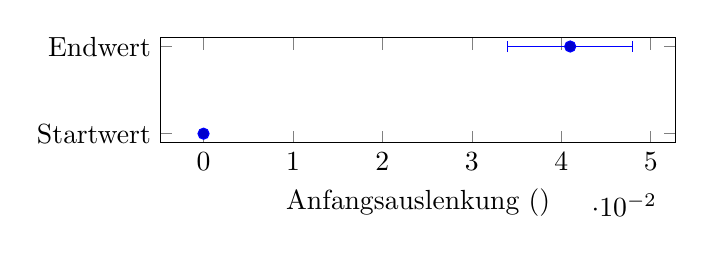
\begin{tikzpicture}
    \begin{axis}[
        try min ticks=2,
        width=.67\textwidth,
        height=.24\textwidth,
        %title = {Vergleich Startwerte und Endwerte: Anfangsauslenkung},
        xlabel = {Anfangsauslenkung ($\si{\meter}$)},
        symbolic y coords = {Startwert,Endwert}
    ]
    \addplot+[
        only marks,error bars/.cd,
        x dir=both,x explicit,
        error bar style={line width=0.5pt},
        ]
    coordinates {
        (0,Startwert)
        (0.041,Endwert) +- (0.007,0)
    };
    \end{axis}
\end{tikzpicture}
\caption{
    Graphischer Vergleich der Start- und Endwerte.
}
\label{fig:pendel:results}
\end{figure}


\clearpage
%-------------------------------------------------------------------------------
\subsection{Tiefpass}
\label{subsec:results:tiefpass}
%-------------------------------------------------------------------------------

Auch bei diesem Versuch stellt die Ermittlung von geeigneten Startwerten f\"ur
die nichtlineare Regression  den haupts\"achlichen Aufwand dar. Da  es sich um
eine  andere  Gesetzm\"assigkeit  als diejenige  der  vorangegangenen  Aufgabe
handelt,  sind  die  dazu  benutzten Methoden  auch  anders. Sie  k\"onnen  im
Abschnitt  \ref{subsubsec:rcglied:startwerte} nachgelesen  werden.  Ein  wenig
vereinfachend ist in diesem Versuch, dass nur eine Gr\"osse gesch\"atzt werden
muss.

Aus   den  gegebenen   Daten   lassen  sich   Regressionen   auf  zwei   Wegen
durchf\"uhren: Einerseits  kann   die  Ausgangsspannung  gegen   die  Frequenz
dargestellt  werden, andererseits  kann dies  aber  auch mit  der Phase  getan
werden. Die beiden Varianten liefern nicht genau die gleichen Ergebnisse f\"ur
die Kapazit\"at $C$.

\begin{center}
\begin{tabular}{lrrr}
    \toprule
                                & Startwert                  & Endwert via Spannung              & Endwert via Phase \\
    \midrule
    Kapazit\"at $C$             &  $\SI{216}{\nano\farad}$   & $\SI{216.8 \pm 0.9}{\nano\farad}$ & $\SI{198 \pm 3}{\nano\farad}$ \\
    \bottomrule
\end{tabular}
\end{center}

\vspace*{2em}
\begin{figure}[th!]
\centering
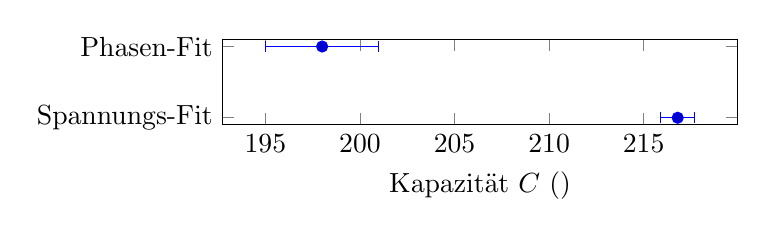
\begin{tikzpicture}
    \begin{axis}[
        try min ticks=2,
        width=.67\textwidth,
        height=.22\textwidth,
        %title = {Vergleich Startwerte und Endwerte: Anfangsauslenkung},
        xlabel = {Kapazit\"at $C$ ($\si{\nano\farad}$)},
        symbolic y coords = {Spannungs-Fit,Phasen-Fit},
    ]
    \addplot+[
        only marks,error bars/.cd,
        x dir=both,x explicit,
        error bar style={line width=0.5pt},
        ]
    coordinates {
        (216.8,Spannungs-Fit) +- (0.9,0)
        (198,Phasen-Fit)      +- (3  ,0)
    };
    \end{axis}
\end{tikzpicture}
\caption{
    Graphischer  Vergleich  der  Werte  f\"ur die  Kapazit\"at  $C$,  bestimmt
    aus  dem Fit  von Ausgangsspannung  and  Frequenz respektive  dem Fit  von
    Phasenverschiebung an Frequenz.
}
\label{fig:rcglied:results}
\end{figure}

Es stehen folgende Punkte hervor:
\begin{itemize}
    \item
        Der Startwert  liegt erstaunlich nahe beim  mittels des Spannungs-Fits
        ermittelten Wert f\"ur die Kapazit\"at $C$.
    \item
        Der mittels Fit von Phase an Frequenz ermittelte Wert f\"ur $C$ weicht
        selbst  mit Ber\"ucksichtigung  der angegebenen  Unsicherheit merklich
        von  den anderen  beiden Werten  ab. Ich  vermute, dass  die Lage  der
        Messpunkte  f\"ur  den Fit  von  Ausgangsspannung  an Frequenz  besser
        geeignet ist,  und dass die  Arkustangens-Funktion des Fits  von Phase
        an   Frequenz  hier  einfach  benachteiligt  ist. Allenfalls  k\"onnte
        durch die  Erh\"ohung der Anzahl Messpunkte  (nat\"urlich bei besserer
        Verteilung) Abhilfe geschaffen werden.
        Es  k\"onnte auch  sein,  dass  der Algorithmus  von  QtiPlot mit  der
        Arkustangens-Funktion  einfach weniger  gut funktionert,  als mit  der
        Division und Quadratwurzel des Zusammenhangs zwischen AusgangsApannung
        und Eingangsspannung  in Abh\"angigkeit  der Frequenz.
        Letztlich  ist  es  nat\"urlich  auch m\"oglich,  dass  der  Startwert
        und  das Resultat  des Spannungs-Fits  weniger korrekt  sind, als  das
        Resultat des Phasen-Fits, allerdings halte  ich dies f\"ur die weniger
        wahrscheinliche Variante,  da diese  beiden Werte so  nahe beieinander
        liegen.
\end{itemize}
